\section{Dokumentation}

Das Backend von \textsc{Kort} ist durchgängig mit der PHP-Dokumentationsprache \emph{PHPDoc}\footnote{\url{http://www.phpdoc.org/}} dokumentiert.
Die Dokumentation findet sich unter: \url{http://kort.herokuapp.com/docs/Kort-backend}

Durch zusätzliche Regeln in unserem Code-Standard (siehe Abschnitt \ref{phpcs}) ist auch sichergestellt, dass die \emph{PHPDoc}-Kommentare stets aktuell sind.

Grundsätzlich stellt die Dokumentation das öffentliche API des Backend dar.
Auch alle anderen Funktionen sind dokumentiert um einen einfachen Einstieg in die Applikation zu ermöglichen.

\begin{figure}[H]
	\centering
	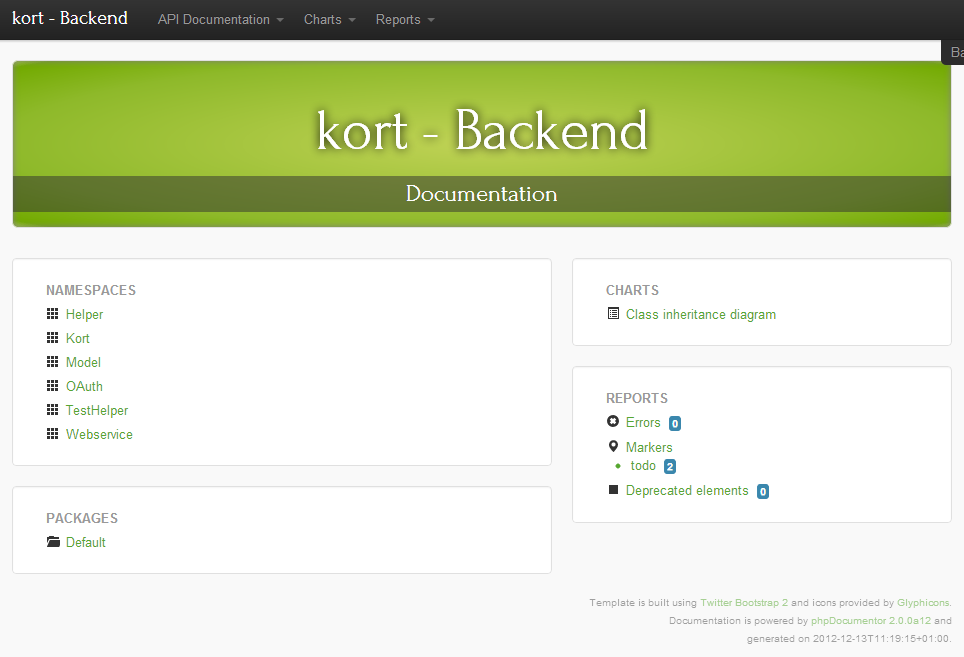
\includegraphics[width=\textwidth]{images/implementation/backend/kort-backend-documentation}
	\caption{Kort Backend Dokumentation mit phpDoc}
	\label{image-kort-backend-documentation}
\end{figure}
